%% Status: 2015-12-30 Some parts collected from wiki.
%% TODO: Describe StellariumScope plugin

\chapter{External Plugins}

\section{StellariumScope plugin}
\label{sec:plugins:StellariumScope}
StellariumScope is a \textbf{free} add-on that enables you to control your telescope with Stellarium. 

The original StellariumScope program was designed and implemented by Scott of ByteArts and is still available for download\footnote{\url{http://www.bytearts.com/stellarium/}}. If you have difficulties with the releases available on Welsh Dragon Computing  site\footnote{\url{http://welshdragoncomputing.ca/x/index.php/home/stellariumscope/about-stellariumscope}}, you may want to consider using the original version.

\paragraph{Features}
\begin{itemize}
\item Provides the interface between Stellarium and the ASCOM telescope drivers.
\item Provides the ability to both ``Sync'' and ``Slew'' the telescope. It's also possible to issue a stop/cancel command from Stellarium.
\item You can easily host Stellarium on one computer linked to another control computer that hosts the telescope driver.
\item The installation program will automatically install the documentation but the link to the documentation is provided here so you can read it before installation.
\item There are earlier releases still available on downloads page on Welsh Dragon Computing  site.
\end{itemize}

\begin{figure}[h]
\begin{center}
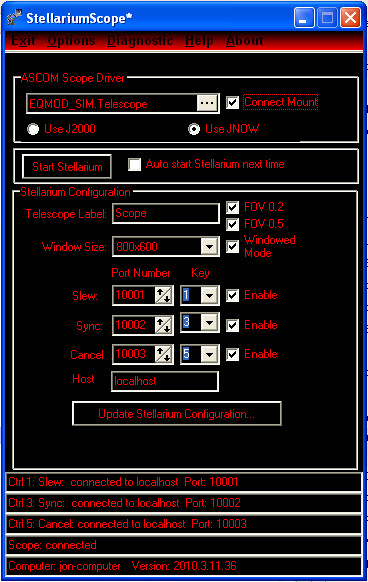
\includegraphics{StellariumScopeFullWindow.jpg}
\end{center}
\label{fig:StellariumScopeFullWindow}
\caption{StellariumScope interface}
\end{figure}

The image \ref{fig:StellariumScopeFullWindow} shows the interface and some of the options.  Use this application (as with all software that controls your mount) with supervision of your mount's movements.

\subsection{Configure StellariumScope}
\label{sec:plugins:StellariumScope:configure}

\subsection{Download StellariumScope}